\documentclass[letterpaper,oneside]{amsart}
\usepackage[T1]{fontenc}
\usepackage{color,soul}
\usepackage[dvipsnames]{xcolor}
\usepackage[utf8]{inputenc}
\usepackage{amsmath}
\usepackage{amssymb}
\usepackage{tikz}
\usepackage{tikz}
\usepackage{amssymb}

\begin{document}

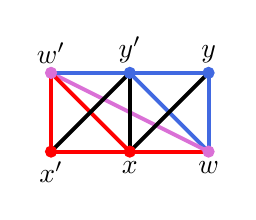
\begin{tikzpicture}
\coordinate (x1) at (0,0);
\coordinate (x2) at (-1,0);
\coordinate (y1) at (1,1);
\coordinate (y2) at (0,1);
\coordinate (w1) at (1,0);
\coordinate (w2) at (-1,1);

\filldraw[black] (x1) circle (0pt) node[anchor=north]{$x$};
\filldraw[black] (x2) circle (0pt) node[anchor=north]{$x'$};
\filldraw[black] (y1) circle (0pt) node[anchor=south]{$y$};
\filldraw[black] (y2) circle (0pt) node[anchor=south]{$y'$};
\filldraw[black] (w1) circle (0pt) node[anchor=north]{$w$};
\filldraw[black] (w2) circle (0pt) node[anchor=south]{$w'$};

\draw[line width=0.5mm,Red] (w1)--(x1);
\draw[line width=0.5mm,RoyalBlue] (w1)--(y1);
\draw[line width=0.5mm,RoyalBlue] (w1)--(y2);
\draw[line width=0.5mm,Orchid] (w1)--(w2);

\draw[line width=0.5mm,Red] (x1)--(x2);
\draw[line width=0.5mm,Black] (x1)--(y1);
\draw[line width=0.5mm,Black] (x1)--(y2);
\draw[line width=0.5mm,Red] (x1)--(w2);

\draw[line width=0.5mm,Black] (x2)--(y2);
\draw[line width=0.5mm,Red] (x2)--(w2);

\draw[line width=0.5mm,RoyalBlue] (y2)--(y1);
\draw[line width=0.5mm,RoyalBlue] (y2)--(w2);

\filldraw[Red] (x1) circle (2pt);
\filldraw[Red] (x2) circle (2pt);
\filldraw[RoyalBlue] (y1) circle (2pt);
\filldraw[RoyalBlue] (y2) circle (2pt);
\filldraw[Orchid] (w1) circle (2pt);
\filldraw[Orchid] (w2) circle (2pt);

\end{tikzpicture}

\end{document}